\documentclass[13pt]{beamer}
%
% Choose how your presentation looks.
%
% For more themes, color themes and font themes, see:
% http://deic.uab.es/~iblanes/beamer_gallery/index_by_theme.html
%
\mode<presentation>
{
\usetheme{CambridgeUS}     % or try Darmstadt, Madrid, Warsaw, ...
\usecolortheme{beaver} % or try albatross, beaver, crane, ...
\usefonttheme{default}  % or try serif, structurebold, ...
\setbeamertemplate{navigation symbols}{}
\setbeamertemplate{caption}[numbered]
} 

\usepackage[english]{babel}
\usepackage[utf8x]{inputenc}
\usepackage{xcolor}
\usepackage{multicol}
\usepackage{tikz}
\usepackage{tikz-uml}
\tikzumlset{font=\footnotesize\ttfamily}
\usepackage{hyperref}

\usepackage{listings}
\definecolor{codegreen}{rgb}{0,0.6,0}
\definecolor{codegray}{rgb}{0.5,0.5,0.5}
\definecolor{codepurple}{rgb}{0.58,0,0.82}
\definecolor{backcolour}{rgb}{0.95,0.95,0.92}

\lstdefinestyle{myCustomCppStyle}{
language=C++,
numbers=left,
stepnumber=1,
numbersep=9pt,
tabsize=2,
showspaces=false,
showstringspaces=false
}

\lstset{basicstyle=\tiny,style=myCustomCppStyle}

\lstdefinestyle{mystyle}{
backgroundcolor=\color{backcolour},   
commentstyle=\color{codegreen},
keywordstyle=\color{magenta},
numberstyle=\tiny\color{codegray},
stringstyle=\color{codepurple},
basicstyle=\ttfamily\footnotesize,
breakatwhitespace=false,         
breaklines=true,                 
captionpos=b,                    
keepspaces=true,                 
numbers=left,                    
numbersep=5pt,                  
showspaces=false,                
showstringspaces=false,
showtabs=false,                  
tabsize=1
}

\lstset{style=mystyle}

\usepackage{graphicx}
\graphicspath{ {./images/} }

\usepackage{tikz}
\usetikzlibrary{decorations.text}
\usetikzlibrary{shapes.geometric, arrows, positioning, calc, matrix}

\tikzset{
basic box/.style={
shape=rectangle, rounded corners, align=center,
draw=#1, fill=#1!25},
header node/.style={
Minimum Width=header nodes,
font=\strut\Large\ttfamily,
text depth=+0pt,
fill=white, draw},
header/.style={%
inner ysep=+1.5em,
append after command={
\pgfextra{\let\TikZlastnode\tikzlastnode}
node [header node] (header-\TikZlastnode) at (\TikZlastnode.north) {#1}
node [span=(\TikZlastnode)(header-\TikZlastnode)] at (fit bounding box) (h-\TikZlastnode) {}
}
},
hv/.style={to path={-|(\tikztotarget)\tikztonodes}},
vh/.style={to path={|-(\tikztotarget)\tikztonodes}},
fat blue line/.style={ultra thick, blue}
}

\definecolor{mygray}{RGB}{208,208,208}
\definecolor{mymagenta}{RGB}{226,0,116}
\newcommand*{\mytextstyle}{\sffamily\Large\bfseries\color{black!85}}
\newcommand{\arcarrow}[3]{%
% inner radius, middle radius, outer radius, start angle,
% end angle, tip protusion angle, options, text
\pgfmathsetmacro{\rin}{1.7}
\pgfmathsetmacro{\rmid}{2.2}
\pgfmathsetmacro{\rout}{2.7}
\pgfmathsetmacro{\astart}{#1}
\pgfmathsetmacro{\aend}{#2}
\pgfmathsetmacro{\atip}{5}
\fill[mygray, very thick] (\astart+\atip:\rin)
                 arc (\astart+\atip:\aend:\rin)
-- (\aend-\atip:\rmid)
-- (\aend:\rout)   arc (\aend:\astart+\atip:\rout)
-- (\astart:\rmid) -- cycle;
\path[
decoration = {
 text along path,
 text = {|\mytextstyle|#3},
 text align = {align = center},
 raise = -1.0ex
},
decorate
](\astart+\atip:\rmid) arc (\astart+\atip:\aend+\atip:\rmid);
}
\title[Design Pattern]{Structural Design Pattern}
\author{Hung Tran}
\institute{Fpt software}
\date{\today}


\begin{document}

\begin{frame}
\titlepage
\end{frame}

% Uncomment these lines for an automatically generated outline.
\begin{frame}{Outline}
\tableofcontents
\end{frame}

\section{Structural Pattern Overview}

\begin{frame}{Structural Pattern Overview}
	\begin{center}
	\textcolor{blue}{\textbf{How classes and objects are composed fo form larger structure.}}
	\end{center}
	\begin{itemize}
		\item \textbf{Adapter}: Convert the interface of a class into another interface.
		\item \textbf{Bridge}: Decouple an abstraction from its implementation.
		\item \textbf{Composite}: Compose objects into tree structure.
		\item \textbf{Decorator}: Attach additional responsibilities to an object dynamically.
		\item \textbf{Façade}: Provide a unified interface to a set of interfaces.
		\item \textbf{Flyweight}: Use sharing to support large numbers of fine-grained objects efficiently.
		\item \textbf{Proxy}: Provide a surrogate or placeholder for another object to control access to it.
	\end{itemize}
\end{frame}

\section{Flyweight pattern}

\begin{frame}{Problem Statement}
\begin{center}
	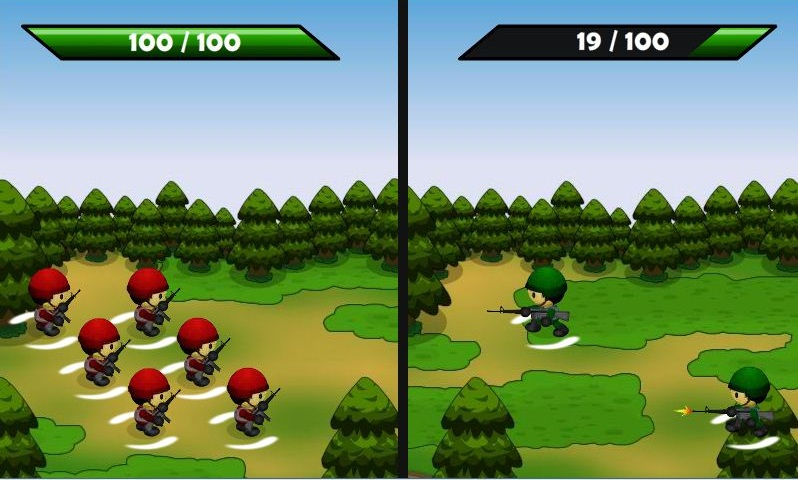
\includegraphics[scale=0.55]{./images/problem.jpg}
\end{center}
\end{frame}

\begin{frame}{Problem Statement}
	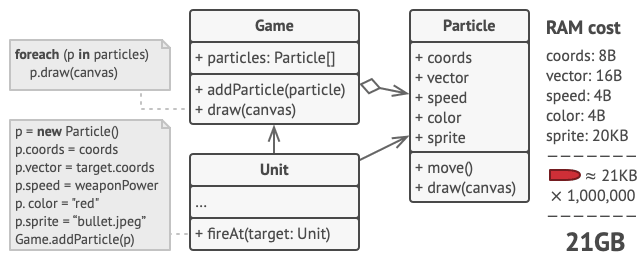
\includegraphics[scale=0.5]{./images/problem1.png}
\end{frame}

\begin{frame}{Problem: Particle class}
	\begin{columns}[T]
		\begin{column}{.5\textwidth}
			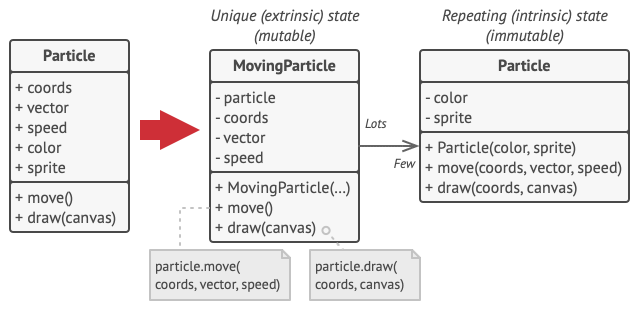
\includegraphics[scale=0.27]{./images/class2.png}
		\end{column}
	
		\begin{column}{.5\textwidth}
			\begin{itemize}
				\item The color and sprite fields consume a lot more memory than other fields.
				\item These two fields store almost identical data across all particles.
				\item For example, all bullets have the same color and sprite.
				\item Coordinates, movement vector and speed, are unique to each particle
			\end{itemize}
		\end{column}
	\end{columns}
\end{frame}

\begin{frame}{Problem: Particle class}
	\begin{itemize}
		\item The intrinsic state: The constant data of an object, the other objects only can read.
		\item The extrinsic state: The other objects can alter these states.
	\end{itemize}
\end{frame}

\begin{frame}{Solution: Flyweight pattern}
	\begin{columns}[T]
		\begin{column}{.5\textwidth}
			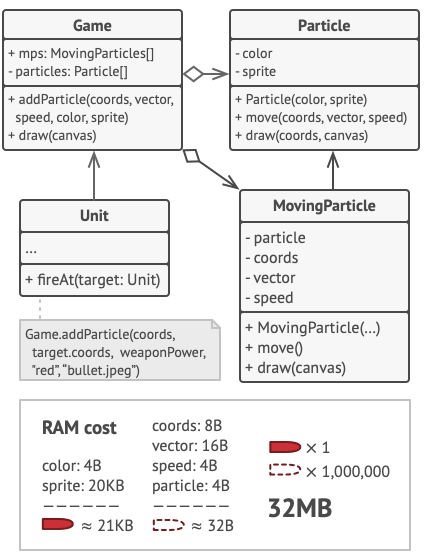
\includegraphics[scale=0.37]{./images/solution.png}
		\end{column}
	
		\begin{column}{.5\textwidth}
			\begin{itemize}
				\item Stop storing the extrinsic state inside the object
				\item Pass this state to specific methods which rely on it.
				\item Only the intrinsic state stays within the object, letting you reuse it in different contexts
				\item Only three different objects would suffice to represent all particles in the game: a bullet, a missile, and a piece of shrapnel.
			\end{itemize}
		\end{column}
	\end{columns}
\end{frame}

\begin{frame}{The Intent of Flyweight Design Pattern}
	\begin{center}
	\textcolor{red}{\textbf{Flyweight is a structural design pattern that lets you fit more objects into the available amount of RAM by sharing common parts of state between multiple objects instead of keeping all of the data in each object.}}\\
	\end{center}
\end{frame}

\begin{frame}{Structure of Flyweight Pattern}
	\begin{center}
	\begin{tikzpicture}
 	\umlclass[x=1,y=0]{FlyweightFactory}{cached : flyweight[]}{GetFlyweight(key)}
 	\umlclass[x=7,y=0]{Flyweight}{}{Operation(extrinsicState)}
 	\umluniaggreg[]{FlyweightFactory}{Flyweight}
 	\umlclass[x=5,y=-3.5]{ConcreteFlyweight}{intrinsicState}{Operation(extrinsic)}
 	\umlclass[x=9.5,y=-3.5]{UnsharedFlyweight}{extrinsicState}{Operation(extrinsic)}
 	\umlinherit[geometry=|-|, pos=0.95, align=right, name=uniassoc]{ConcreteFlyweight}{Flyweight}
 	\umlinherit[geometry=|-|, pos=0.95, align=right, name=uniassoc]{UnsharedFlyweight}{Flyweight}
 	\umlclass[x=1,y=-5]{Client}{}{}
 	\umluniassoc[]{Client}{FlyweightFactory}
 	\umluniassoc[geometry=-|]{Client}{ConcreteFlyweight}
 	\umluniassoc[geometry=-|]{Client}{UnsharedFlyweight}
	\end{tikzpicture}	
	\end{center}
\end{frame}

\begin{frame}{Applicability}
	\begin{itemize}
		\setlength\itemsep{1em}
		\item  Use the Flyweight pattern only when your program must support a huge number of objects which barely fit into available RAM.
		\item The benefit of applying the pattern depends heavily on how and where it’s used. It’s most useful when:
		\item An application needs to spawn a huge number of similar objects
		\item This drains all available RAM on a target device
		\item The objects contain duplicate states which can be extracted and shared between multiple objects
	\end{itemize}
\end{frame}

\begin{frame}{How to Implement}
	\begin{itemize}
		\setlength\itemsep{1em}
		\item Divide fields of a class that will become a flyweight into two parts: the intrinsic state and the extrinsic state
		\item Leave the fields that represent the intrinsic state in the class, but make sure they’re immutable. They should take their initial values only inside the constructor.
		\item Go over methods that use fields of the extrinsic state. For each field used in the method, introduce a new parameter and use it instead of the field.
		\item Optionally, create a factory class to manage the pool of flyweights. It should check for an existing flyweight before creating a new one. Once the factory is in place, clients must only request flyweights through it. They should describe the desired flyweight by passing its intrinsic state to the factory.
		\item The client must store or calculate values of the extrinsic state (context) to be able to call methods of flyweight objects. For the sake of convenience, the extrinsic state along with the flyweight-referencing field may be moved to a separate context class.
	\end{itemize}
\end{frame}

\begin{frame}{Pros and Cons}
	\begin{columns}[T]
		\begin{column}{.5\textwidth}
			\begin{itemize}
				\item You can save lots of RAM, assuming your program has tons of similar objects.
			\end{itemize}
		\end{column}
	
		\begin{column}{.5\textwidth}
			\begin{itemize}
				\item You might be trading RAM over CPU cycles when some of the context data needs to be recalculated each time somebody calls a flyweight method.
				\item The code becomes much more complicated. New team members will always be wondering why the state of an entity was separated in such a way.
			\end{itemize}
		\end{column}
	\end{columns}
\end{frame}

\begin{frame}{Relations with Other Patterns}
	\begin{itemize}
		\setlength\itemsep{1em}
		\item You can implement shared leaf nodes of the Composite tree as Flyweights to save some RAM.
		\item Flyweight shows how to make lots of little objects, whereas Facade shows how to make a single object that represents an entire subsystem.
		\item Flyweight would resemble Singleton if you somehow managed to reduce all shared states of the objects to just one flyweight object. But there are two fundamental differences between these patterns:
		\item There should be only one Singleton instance, whereas a Flyweight class can have multiple instances with different intrinsic states.
		\item The Singleton object can be mutable. Flyweight objects are immutable.
	\end{itemize}
\end{frame}

\begin{frame}
\begin{center}
{\fontsize{40}{50}\selectfont Thank You!}
\end{center}
\end{frame}

\end{document}
